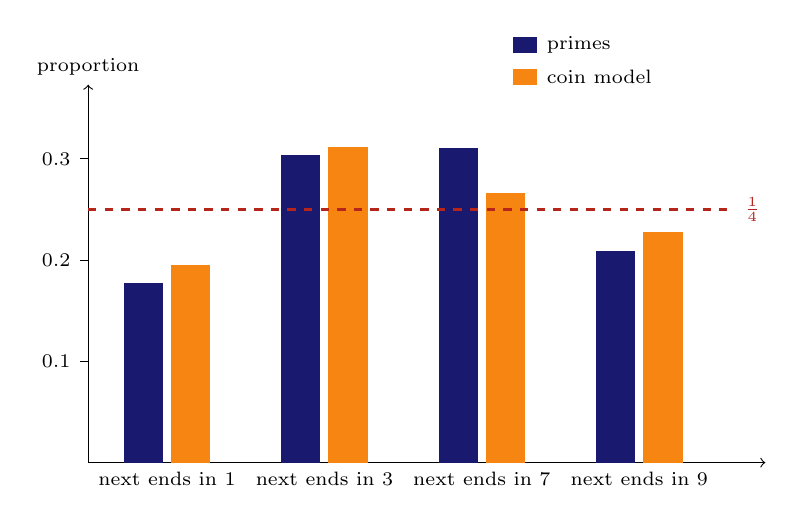
\begin{tikzpicture}[x=1cm,y=1cm]
\draw[->] (0,0) -- (8.6,0);
\draw[->] (0,0) -- (0,4.800) node[above] {\scriptsize proportion};
\draw (0,1.286) -- (-0.1,1.286) node[left] {\scriptsize $0.1$};
\draw (0,2.571) -- (-0.1,2.571) node[left] {\scriptsize $0.2$};
\draw (0,3.857) -- (-0.1,3.857) node[left] {\scriptsize $0.3$};
\fill[MidnightBlue] (0.45,0) rectangle (0.95,2.2757);
\fill[BurntOrange] (1.05,0) rectangle (1.55,2.5041);
\node[below] at (1.00,0) {\scriptsize next ends in $1$};
\fill[MidnightBlue] (2.45,0) rectangle (2.95,3.9076);
\fill[BurntOrange] (3.05,0) rectangle (3.55,4.0028);
\node[below] at (3.00,0) {\scriptsize next ends in $3$};
\fill[MidnightBlue] (4.45,0) rectangle (4.95,3.9900);
\fill[BurntOrange] (5.05,0) rectangle (5.55,3.4228);
\node[below] at (5.00,0) {\scriptsize next ends in $7$};
\fill[MidnightBlue] (6.45,0) rectangle (6.95,2.6838);
\fill[BurntOrange] (7.05,0) rectangle (7.55,2.9274);
\node[below] at (7.00,0) {\scriptsize next ends in $9$};
\draw[BrickRed,thick,dashed] (0,3.2143) -- (8.2,3.2143) node[right] {\scriptsize $\frac14$};
\fill[MidnightBlue] (5.4,5.2) rectangle (5.7,5.4); \node[right] at (5.7,5.3) {\scriptsize primes};
\fill[BurntOrange] (5.4,4.8) rectangle (5.7,5.0); \node[right] at (5.7,4.9) {\scriptsize coin model};
\end{tikzpicture}
